%%********DO NOT EDIT****************
\documentclass[12pt]{article}
\usepackage[utf8]{inputenc}  %%% added 
\usepackage{mathptmx}
\usepackage{graphicx}
\usepackage{grffile} %%% added
\pagestyle{empty}

\setlength\topmargin{0pt}
\addtolength\topmargin{-\headheight}
\addtolength\topmargin{-\headsep}
\setlength\oddsidemargin{0pt}
\setlength\textwidth{\paperwidth}
\addtolength\textwidth{-2in}
\setlength\textheight{\paperheight}
\addtolength\textheight{-2in}
\usepackage{layout}

\renewcommand{\title}[1]{\noindent\textbf{#1}\bigskip\\}
\renewcommand{\author}[1]{\noindent #1\bigskip\\}
%%***********************************

\begin{document}

%**********USER DEFINED**************
\title{The Problem of Action at a Distance in Networks and the Emergence of Preferential Attachment from Triadic Closure}
%Enter author(s) and address here
\author{Jérôme Kunegis,$^1$ Fariba Karimi,$^2$ and Jun Sun$^3$\bigskip\\
{\small
1. Université de Namur, Belgium\\
2. GESIS -- Leibniz-Institut für Sozialwissenschaften, Germany \\
3. Universität Koblenz--Landau, Germany 
}
}
%Enter abstract here
We discuss the notion of action at a distance in networks, in the
context of graph growth models. 
Action at a distance is a notion
from physics that refers to certain interactions (forces) seemingly
acting between objects that are far from each other, independently of
any intervening matter.  In the network setting, the analogous
phenomenon refers to graph models in which edges are created between
nodes that are seemingly far from each other, without taking into
account the network structure between them. 
In particular, we argue that
preferential attachment represents a form of action at a distance that
can be explained as an emergent phenomenon in the context of triangle
closing, thus allowing us to explain real-world graph growth without
inherent action at a distance. To support our claims, we present both theoretical and
experimental evidence. 

As theoretical evidence, we show that
preferential attachment arises in the limit of a particular random graph model in
which triangle closing is allowed.  The derivation is exact in the limit
when the number of nodes goes to infinity, and takes a random process of
triangle closing as a starting assumption. 

Experimentally, we show evidence for preferential attachment in a continuum of random graph
models that include only local graph growth rules.  Specifically, we
explore graph models that include triangle closing.  We test our results
statistically by comparing them with complete random graphs
(Erdős--Rényi) and preferential attachment models (e.g.,
Barabási--Albert). 

\begin{figure}[!h]
\begin{center}
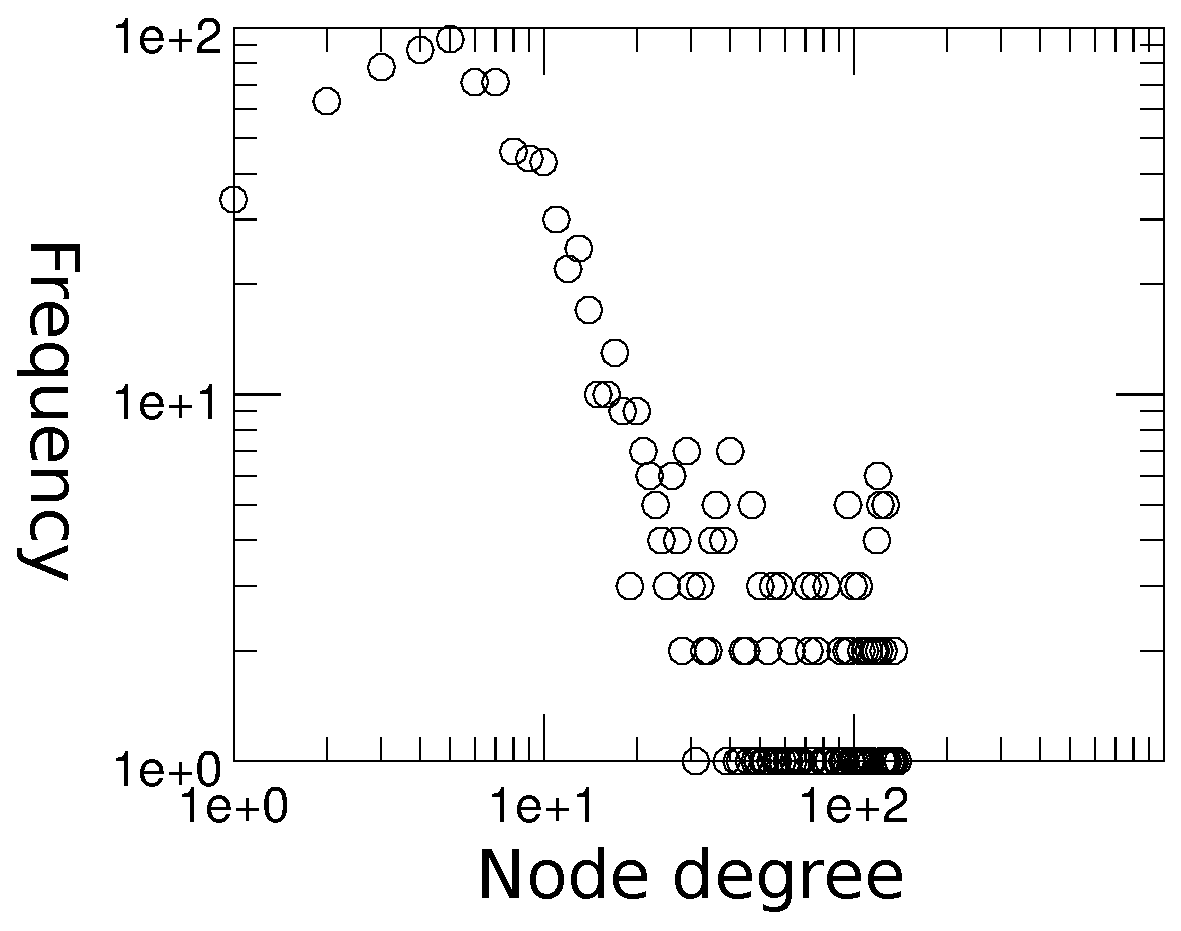
\includegraphics[scale=0.4]{degree.triangle.edited}
\end{center}
\caption{
  The degree distribution of a synthetic graph based on a graph growth
  model using only local graph growth rules.  Despite the lack of
  preferential attachment in the graph model, the resulting graph
  displays scale-free behavior, an example of what we characterize to
  be, in the paper, action at a distance. 
}
\end{figure}
% Place the abstract of your talk/poster here, 250 Words maximum.
% Mathematical formulae may be set in LaTeX, but do NOT use the
% bibliography environment -- if you must have references, use an 
% enumerated list.
%
% Your abstract (plus one figure) should not exceed one page.
%
% Check carefully.

%************************************
\end{document}
